


In this part of the homework we use the QR-factorization to solve a square ill-conditioned system. We use the given function \texttt{illposed.m} to generate an ill-conditioned system of size 8. 

\paragraph*{a) Estimate condition number of a linear system}

Given the matrix $A$, we can introduce a perturbation $b+\Delta b$ to estimate the condition number of $A$ with 
$$\dfrac{\parallel \Delta x \parallel_2}{\parallel x \parallel_2}\leq\kappa (A)\dfrac{\parallel \Delta b \parallel_2}{\parallel b \parallel_2}.$$

We took a large number of random perturbations and kept the one that gave the largest estimation of the condition number. The estimation of the condition number for a matrix $A$ is in the table below. Taking another random matrix $A$ give very similar results. 

\begin{table}[hb]
\centering
\begin{tabu}{|c|c|}
\hline 
\texttt{cond(A)} & \texttt{estimateCond(A)} \\ 
\hline 
1.67e+12 & 5.05e+11 \\ 
\hline 
\end{tabu}
\caption{Estimated condition number of A compared with Matlab}
\end{table} 
It is clear that we find a lower bound of the exact condition number since we can only try a finite number of perturbations.


\paragraph*{b) Approximate solution of an ill-posed system}

The script \texttt{qrFact.m} solves the task at hand. We solve the system for different values of the rank $r$. We define the residual $\txt{res} = A\hat{x}-b$. Each time we estimate the condition number of $R_{11}$ to compare it with the value of the Matlab function \texttt{cond}. We compute other values that appear in the table below.

\begin{center}
\begin{tabular}{|c|c|c|c|c|c|}
\hline 
rank $r$ & $\parallel E\parallel$  & $\parallel res \parallel$ &  cond(R11) & estimationCond(R11) & $\parallel \hat{x} \parallel$ \\ 
\hline 
8 & /                  & $8.8818*10^{-16}$     & $1.6882*10^{12}$ & $0.8736*10^{12}$      &  1.701 \\ 
\hline 
7 & $5.3835*10^{-12}$                  & $0.3267*10^{-11}$ & $2.8435*10^{9}$ & $1.2983*10^{9}$ &  2.202 \\ 
\hline 
6 & $0.2064*10^{-8}$         & $0.2878*10^{-9}$ & $10.8204$        & 5.3686 &  3.212 \\ 
\hline 
5 & $0.5647$     & 0.4753       & 6.8978  & 3.2608 &  2.676 \\ 
\hline 
\end{tabular} 
\end{center} 

Let's analyze the different numerical relations. The value $\parallel E \parallel$ increases as the rank decreases. This makes perfect sense since when decreasing the rank we set more elements to zero and $E$ has more entries. On the other hand, decreasing the rank reduces the quality of the approached solution and thus we get a larger residual. We commit a less accurate approximation by setting more elements to zero. We can note that the norm of the residual should be zero for $r=8$ (as we solve the system exactly). The value obtained (around $10^{-16}$) is due to floating point errors and should be considered zero.

For the estimation of the condition number, we have again a lower bound of the exact value (let's assume that the value given by Matlab is close enough to the exact value). We are not so far away from the value of Matlab. At least the tendency of the condition number with $r$ is correct as we also see on the two lower graphs of figure~\ref{qr}. This number is decreasing as the rank decreases. This again makes sense because the whole point of setting entries to zero is to solve a problem that is less sensitive. Finally the norm of the solution $\hat{x}$ is not related to the rank $r$. We just note that the steps applied lead to the solution with the smallest norm (since the problem with modified rank does not have an unique solution).

On figure \ref{qr}, we can see that the "best" choice for $r$ is $6$. We can see that for this value, the condition number is quite small (around $10^1$) and the approximation is quite good because the norm of the residual is around $10^{-10}$. This seems to be the best trade-off between the quality of the approximation and the sensitivity of the solution.

\begin{figure}
\begin{center}
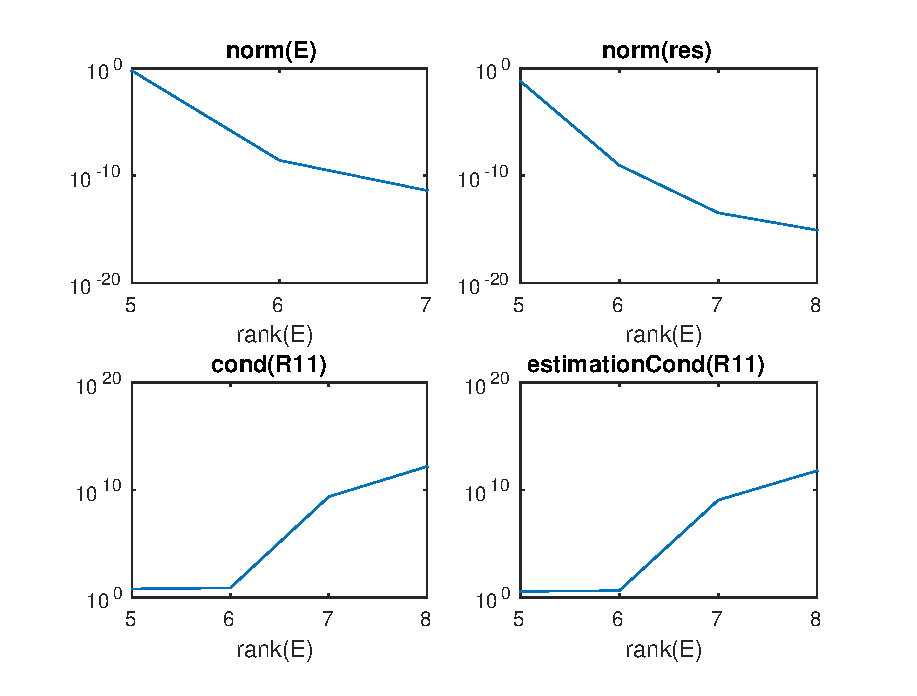
\includegraphics[scale=0.7]{qrPlot.eps}
\caption{Numerical relations as a function of the rank $r$}
\label{qr}
\end{center}
\end{figure}

\FloatBarrier







